%********************************************************************************************
%								COMANDOS ÚTILES PARA LATEX EN ESTE TP							
%
%	\ : espacio simple
%	\\ : nueva línea
%	\par : va a la línea de abajo y deja sangría
%	\vspace{##tamaño en pt##} o \vspace{\baselineskip} en general:
%								 para dejar un espacio vertical
%	\textbf{text} :text en negrita
%	\textit{text} :text en itálica
%
% GRAFICOS CENTRADOS:
%	\begin{center}
%		\includegraphics[width=\textwidth]{./img/##ruta imagen (no hace falta extension)##}
%	\end{center}
%		--> se pueden agregar atributos como scale por si se hace muy grande
%
% TABLAS CENTRADAS:
%	\begin{center}
%	\begin{tabular}{|c|c|}
%	\hline
%	\ \textbf{Programa} & \textbf{Ticks} \\
%	\hline
%		ASM & 675127609 \\
%	\hline
%	\end{tabular}
%	\end{center}
%
% ALGORITMOS (EN VARIOS LENGUAJES):
% \begin{lstlisting}
%	void sumoDiez(int &num)
%	{
%	    num += 10;
%	}
%	
%	int main()
%	{
% 	   int i;
%	    int numeroAProcesar = 20;
%	    for (i = 0; i < 50; i++)
%	    {
%	        sumoDiez(numeroAProcesar);	//Proceso el numero en cada ciclo
%	    } 
%	    return 0;
%	}
%	\end{lstlisting}
%
% para info sobre todo lo que tiene el package detallado:
% http://en.wikibooks.org/wiki/LaTeX/Source\_Code\_Listings
%
%********************************************************************************************

\documentclass[10pt,a4paper]{article}
\usepackage[utf8]{inputenc} % para poder usar tildes en archivos UTF-8
\usepackage[spanish]{babel} % para que comandos como \today den el resultado en castellano
\usepackage{a4wide} % márgenes un poco más anchos que lo usual
%\usepackage{geometry}

%\usepackage{layout}

%\geometry{
%  includeheadfoot,
%  margin=2.7cm
%}

\usepackage[conEntregas]{caratula}
\usepackage{amssymb}
\usepackage{fancybox}
\usepackage[usenames,dvipsnames]{color}
\usepackage{hyperref}
\usepackage{listings}
\usepackage{clrscode3e}
\usepackage{xcolor}
\usepackage{amsmath}


\hypersetup{
    colorlinks,
    citecolor=black,
    filecolor=black,
    linkcolor=black,
    urlcolor=black
}

\lstdefinestyle{customc}{
  belowcaptionskip=1\baselineskip,
  breaklines=true,
  frame=L,
  xleftmargin=\parindent,
  language=C,
  showstringspaces=false,
  basicstyle=\footnotesize\ttfamily,
  keywordstyle=\bfseries\color{green!40!black},
  commentstyle=\itshape\color{purple!40!black},
  identifierstyle=\color{blue},
  stringstyle=\color{orange},
}

\lstset{escapechar=@,style=customc}

\begin{document}

\titulo{Trabajo Práctico 2}
\subtitulo{Tirate un qué, tirate un ranking... [Primera entrega]}

\fecha{\today}

\materia{Métodos Numéricos}
\grupo{Grupo Autodenominado "Los Pichis"}

\integrante{De Sousa Bispo, Germán Edgardo}{359/12}{german\_nba11@hotmail.com}
\integrante{De Sousa Bispo, Mariano Edgardo}{389/08}{marian\_sabianaa@hotmail.com}
\integrante{Valdés Castro, Tobías}{800/12}{tobias.vc@hotmail.com}


\maketitle

\tableofcontents
\newpage

\section*{Introducción}
\addcontentsline{toc}{section}{Introducción}

Los talentosos y apuestos muchachos que instauraron la moda de los cabellos raros y los pasos bailables más utilizados en los últimos años han caído lentamente en el olvido. Con el fin de volver a su momento de gloria, el grupo tropical ha contactado al DC para brindarles una solución teniendo en cuenta el bajo presupuesto con el que cuentan en el momento.

Los motores de búsqueda son herramientas claves para explorar la red. Lo único que debemos hacer para utilizarlos es enviar un \textit{query} con lo que querramos buscar, y allí el motor se encargará de darnos la información correspondiente a nuestra búsqueda. Para que la experiencia del usuario sea óptima, esta información \textit{no puede estar presentada de cualquier forma}. Por lo tanto, una tarea vital del buscador será devolver al usuario un listado de páginas cuyo orden será impuesto por la \textit{relevancia} de cada página. 

El equipo de Métodos Númericos ha llegado entonces a la siguiente conclusión:  para volver a todos los televisores nacionales e internacionales, este grupo de genios musicales debe figurar en páginas importantes en la web (y así encabezar todas las búsquedas). El problema ahora radica en determinar cuáles son las páginas importantes que posicionarán al grupo en los primeros links de cualquier búsqueda tropical. 

De esta manera, el grupo autodenominado ``Los Pichis'' comenzó la labor de estudiar algunos de los más conocidos algoritmos de búsqueda: \textit{In-Degree}, \textit{PageRank} y \textit{Hyperlink-Induced Topic Search}(HITS).

El primero se basa en generar el ranking de importancia de la web teniendo en cuenta solamente la cantidad de links que apuntan a la página. Mientras mayor sea la cantidad de links, más importante es la página. 

\textit{PageRank} es un algoritmo que luego de buscar en toda la red e indexar los datos obtenidos para realizar una búsqueda eficiente, rankea la importancia de la base de datos de manera que, cuando el usuario realiza una búsqueda, las páginas más importantes se presenten primero. Si una página $u$ apunta a una página $v$, se puede decir que $v$ es importante. Sin embargo, para no dejar que simplemente una página sea más importante por tener muchas páginas apuntadas a ella, se puede realizar un ponderado de los links utilizando la importancia de la página de origen (no es lo mismo ser apuntado por una página importante que por muchas no importantes). De esta manera, consideramos la importancia de una página $v$ como la importancia de la página $u$ (que apunta a $v$) e inversamente proporcional al grado de $u$ (es decir, la cantidad de links que  posee la página $u$). Entonces, si la página $u$ contiene $n_u$ links, uno de los cuales apunta a $v$, el aporte de ese link a la página $v$ será $x_u / n_u$.
Como para cada página pedimos la siguiente ecuación: 
\begin{eqnarray}
x_k = \sum_{j \in L_k} \frac{x_j}{n_j},~~~~k = 1,\dots,n. \label{eq:basicmodel}
\end{eqnarray}
Luego, el modelo planteado es equivalente a encontrar un $x\in \mathbb{R}^n$ tal que $Px = x$. Esto significa, encontrar un autovector asociado al autovalor 1 de una matriz cuadrada, tal que $x_i \ge
0$ y $\sum_{i = 1}^n x_i = 1$.
\par 
Finalmente, la idea del método \textit{HITS} se basa en una noción de autoridad que se trasmite de una página a otra mediante links. Es decir, se considera que existen páginas que cumplen rol de autoridad sobre un tema y se trata de modelar la relación entre estas páginas y aquellas que las apuntan, las cuales se denominan \textit{hubs}. 
La relación entre ambos se establece matricialmente de la siguiente forma: 

\begin{eqnarray}
x & = & A^ty \label{eq:auth-update-math} \\
y & = & Ax, \label{eq:hub-update-math} 
\end{eqnarray}

Siendo $x$ un vector de peso de autoridad, $y$ el de los hubs y $A$ la matriz de adyacencia creada a partir de los links de una página a otra.
Kleinberg propone en \textit{Authoritative sources in a hyperlinked environment} con un $y_0$ inicial, al cual aplicarle esta ecuación iterativamente para que, bajo ciertas condiciones que nuestro problema cumple, el método converja. En base a este ranking obtenido luego de realizar las iteraciones, se obtienen las páginas que son mejores autoridades y mejores hubs.




aplicando luego el paso de normalizaci\'on correspondiente. Los autores proponen comenzar con un $y_0$ incial, aplicar estas ecuaciones 
iterativamente y demuestran que, bajo ciertas condiciones, el m\'etodo converge. Finalmente, en base a los rankings obtenidos, se retorna
al usuario las mejores $t$ \emph{autoridades} y los mejores $t$ \emph{hubs}.


\section{Desarrollo}
\subsection{Ideas sobre la Implementación}

\subsubsection{Características generales del problema}


\subsection{Implementación}

	En la implementación, decidimos utilizar herencia y polimorfismo para simplificar el código. Este trabajo práctico es significativamente más grande que el anterior; una implementación descuidada necesariamente nos conduciría a muchos errores, complejos de encontrar y corregir. 

	Los puntos centrales tenidos en cuenta para el desarrollo fueron:

	\begin{itemize}
		\item \textbf{Algoritmos}: Debemos implementar tres algoritmos distintos para buscar prácticamente la misma información: \textit{Page Rank, HITS, In Degree}
		\item \textbf{Parsing}: El parseo de los archivos de inputs deben ser distintos dependiendo de su instancia: \textit{Stanford, Toronto}
		\item \textbf{Declaratividad}: Nos es más fácil pensar el problema si tenemos una \texttt{WebNet} y un conjunto de \texttt{WebPage} para aplicar los algoritmos, las cuales poseen a su vez \texttt{Rank} . En el único momento que efectivamente necesitamos sus valores (por ejemplo cantidad de nodos con los que se conecta) es para aplicar el método de la potencia. De esta manera la implementación de las operaciones de matriz quedan ocultas dentro de cada algoritmo de \textit{ranking}.
	\end{itemize}

	Escribiendo un pseudo-código, el punto de entrada \textit{(main)} de nuestra aplicación es muy similar al siguiente:

	\vspace{\baselineskip}
	\begin{codebox}
	\Procname{$\proc{PageRanking}()$}
	\li ParsingAlgorithm \id{parsingAlgorithm} = createParsingAlgorithmFromParameters(entryPointParameters)
	\li WebNet \id{net} = parsingAlgorithm.parseFile(webDefinitionFile)
	\li RankingAlgorithm \id{rankingAlgorithm} = createRankingAlgorithmFromParameters(entryPointParameters)
	\li rankingAlgorithm.RankPages(net)
	\li parsingAlgorithm.SaveRank(net)
	\End
	\end{codebox} 
	\vspace{\baselineskip}

	Como se comentó anteriormente, es necesario para \textit{Page Rank} y \textit{HITS} aplicar un método iterativo para obtener el \textit{ranking} que buscamos. En este trabajo, utilizamos el método de la potencia. 

	Por otro lado, sabemos que la red generada por la interconexión entre páginas genera un grafo donde el grado de cada nodo rara vez es \textit{n} (siendo \textit{n} la cantidad de páginas). Por lo tanto, generar la matriz de adyacencia no parece ser una buena solución: tendríamos muchos elementos cuyo valor es cero. La cátedra sugirió tres posibles implementaciones de matrices esparsas: \textit{Dictionary of keys (DOK)}, \textit{Compressed Sparse Row (CSR)} y \textit{Compressed Sparse Column (CSC)}. Nosotros optamos por \textit{CSR}, y la justificación la detallamos a continuación.

\subsubsection{Implementación con matriz Column Sparse Row (CSR)}

	Definamos como \textit{n} a la cantidad de columnas y filas de la matriz, \textit{CSR} la almacena utilizando únicamente tres arreglos (sean: \textit{rowPointers, colIndexes y values}), la dimensión de ellos son: \textit{n} para \textit{rowPointers}, cantidad de elementos no nulos para \textit{colIndexes} e igual cantidad para \textit{values}.

	La semántica de estos arreglos es la siguiente, suponiendo que \textit{i} hace referencia a filas y \textit{j} a columnas:

	\begin{itemize}
		\item \texttt{rowPointers}: El valor de la i-ésima posición referencia el índice de colIndexes a partir del cual se encuentran los elementos de la i-ésima fila. En caso de no haber elementos en la i-ésima fila de la matriz, esta posición se completa con el mismo valor que la i-1 (simplemente por cuestiones implementativas). Este vector tendrá entonces $m+1$ elementos para poder representar a las $m$ filas, y además el primer elemento siempre será 0 (índice en base 0) y el último siempre será la cantidad de valores no nulos.
		\item \texttt{colIndexes}: El valor contenido dentro de cada posición representa a \textit{j}
		\item \texttt{values}: Contiene los valores de la matriz, cada posición se relaciona uno a uno con \textit{colIndexes}. Se puede deducir fácilmente entonces que el tamaño de este vector es igual al de \texttt{colIndexes}.
	\end{itemize}
	
	Veamos entonces un ejemplo del guardado de una matriz $A$ para esta estructura de datos:
\[	A =
	 \begin{pmatrix}
	 0 & 1 & 0 & 0 & 5 \\
	 2 & 3 & 0 & 0 & 1 \\
	 0 & 0 & 0 & 0 & 0 \\
	 0 & 0 & 0 & 7 & 0 \\
	 8 & 0 & 11 & 0 & 4
	 \end{pmatrix}
\]	

	\begin{itemize} 
 \item Para \texttt{values}, debemos recolectar todos los valores no nulos en orden izquierda-derecha-arriba-abajo: \texttt{values} $= [1,5,2,3,1,7,8,11,4].$

 \item Para \texttt{colIndexes}, debemos recolectar todos las columnas de esos valores y ponerlas en el mismo orden que en \texttt{values}. Luego (en base 0): \texttt{colIndexes} $= [1,5,2,3,1,7,8,11,4].$

 \item Finalmente para \texttt{rowPointers}, siendo este el más difícil de entender, debemos guardar en \texttt{rowPointers[$i$]} y \texttt{rowPointers[$i+1$]} el rango de índices\footnote{Rango final \textbf{no} incluído.} de \texttt{colPointers}\footnote{Se puede mirar también en \texttt{values}.} en el cual hay valores en la fila $i$ (en base 0). 
 
 En el ejemplo vemos lo siguiente: en la primera fila hay 2 valores no nulos, por lo tanto \texttt{rowPointers[0] = 0, rowPointers[1] = 2}. Esto indica entonces que mi primera fila tiene los valores en \texttt{values} del índice 0 al índice 2 (no incluído), es decir el 1 y el 5 (cuyas columnas aparecen en \texttt{colIndexes} para esos mismos índices). Siguiendo el ejemplo, tendría \texttt{rowPointers} $ = [0,2,5,5,6,9]$. 
 
 De esto se puede notar que efectivamente el tamaño de este vector es de la cantidad de filas más 1. También se puede ver que se repite el número 5 para los índices 2 y 3 de este vector: esto quiere decir que en la fila 2 (la tercera) debería mirar desde el índice 5 al 5 (\textbf{no} incluído) en los otros dos vectores de columnas y valores, y evidentemente eso no es posible por lo cual no hay ningún valor en esa fila.
 
 Una manera fácil de ver el llenado de este vector es poner en \texttt{rowPointers[i]} la sumatoria de la cantidad de elementos no nulos hasta la fila $i$: hasta la fila de índice 0, hay 0 elementos. Hasta la fila 1, hay 2. Siguiendo este razonamiento, hasta la fila 2 hay 5 elementos. En la fila 3 sigue habiendo 5 elementos ya que no apareció ningún otro no nulo. En la fila 4 hay sólo uno más luego hasta ella hay 6 elementos, y finalmente llego a que hasta la última fila encontré todos mis 9 valores no nulos.
		\end{itemize}

	Si queremos obtener el elemento $a_{ij}$, podemos definir el siguiente pseudo-codigo:

	\vspace{\baselineskip}
	\begin{codebox}
	\Procname{$\proc{Element}(i, j)$}
	\li int \id{colIndexLower} = rowPointers[i]
	\li int \id{colIndexUpper} = rowPointers[i+1]
	\li \For $col \gets colIndexLower$ \To $colIndexUpper$ \Do
	\li \If  colIndexes[col] == j
	\li \Then return values[col]
	\End
	\End
	\End
	\end{codebox} 
	\vspace{\baselineskip}
	
	La multiplicación entre una matriz con esta implementación y un vector se realiza entonces sencillamente siguiendo la misma idea: iterando las filas desde \texttt{rowPointers[i]} a \texttt{rowPointers[i+1]} como en el pseudocódigo anterior, multiplicamos únicamente las posiciones \textit{j} del vector que tengamos en \texttt{colIndexes} por el valor almacenado en values. Si ninguna multiplicación es efectuada, el valor el cero. Este algoritmo de multiplicación es \textit{un paso clave} para desarrollo de los algoritmos de búsqueda propuestos. Veamos lo que sucede matemáticamente con este tipo de matrices: 

\vspace{\baselineskip}

\[	Av =
	 \begin{pmatrix}
	 0 & a_{1,2} & 0 & 0 & a_{1,5} \\
	 a_{2,1} & a_{2,2} & 0 & 0 & a_{2,5} \\
	 0 & 0 & 0 & 0 & 0 \\
	 0 & 0 & 0 & a_{4,4} & 0 \\
	 a_{5,1} & 0 & a_{5,3} & 0 & a_{5,5}
	 \end{pmatrix}
	 \cdot
	 \begin{pmatrix}
	 v_1 \\
	 v_2 \\
	 v_3 \\
	 v_4 \\
	 v_5 
	 \end{pmatrix}
	  = filas(A) \cdot v
\]
\vspace{2 pt}
\[
	= 0 \times v_1 + a_{1,2} \times v_2 + 0 \times v_3 + 0 \times v_4 + a_{1,5} \times v5 + ... + 0 \times v_4 + a_{5,5} \times v_5
\]
\vspace{2 pt}
\[
    = \sum a_{i,j} v_j  \ \ \ \ \ \ \ \ (\forall a_{i,j} \neq 0)
\]
\vspace{5 pt}

\par
Asi que básicamente en palabras lo que sucede es que \textit{todos los términos que son 0 en la matriz esparsa no se tienen en cuenta para la multiplicación} porque al ser el elemento neutro de la suma no producen ningún cambio. Además sabemos, por las propiedades de la multiplicación entre matrices y vectores, que \textit{aquellos términos $a_{i,j}$ que no sean 0 estarán multiplicados por $v_j$}. 

Mirando ahora como está hecha la estructura de las matrices esparsas con \textit{CSR}, podemos ver que conocemos cada columna de cada valor no nulo (en \texttt{colIndexes}), cuáles son esos valores (\texttt{values}) y en qué fila están (analizando apropiadamente \texttt{rowPointers}). Teniendo esto en cuenta, el pseudocódigo (o algoritmo directamente) para la multiplicación con la implementación \textit{CSR} es el siguiente:

	\vspace{\baselineskip}
	\begin{codebox}
	\Procname{$\proc{MatrixVectorMultiplication}$(vector $v)$}
	\li vector \id{multiplicationVector}
	\li \For $i \gets 0$ \To $m$ \Do
	\li \id{rowValue} $\gets$ 0
	\li \For $j \gets rowPointers[i]$ \To $rowPointers[i+1]$ \Do
	\li $rowValue += values[j] \times v[colIndexes[j]]$  \End 
	\li
	\li $multiplicationVector$.pushToVector($rowValue$); \End
	\li 
	\li return $multiplicationVector$
	\End
	\end{codebox} 
	\vspace{\baselineskip}

\par	
Por la naturaleza de la multiplicación de matriz por vector, resulta poco conveninete utilizar la estructura \textit{CSC}. \textit{CSC} es más redituable si necesitamos multiplicar por la traspuesta de una matriz, ya que el mismo algoritmo la recorrería de manera traspuesta\footnote{En el algoritmo de \textit{HITS} necesitamos la traspuesta, sin embargo, utilizamos la misma estructura, cargando los índices de manera inversa.}.

	Tanto \textit{CSR} como \textit{CSC} son complejos de crear si los datos no son suministrados de manera ordenada. Para eso, generamos una clase \textit{CSRBuilder} al cual se le pasan los datos de manera desordenada y una vez que la carga de datos se completa, se encarga de ordenarlos, crear los índices e instanciar una \textit{CSRMatrix}. Si bien no es idéntico, preserva el espíritu de un \textit{DOK}, ya que termina utilizando de cláve \textit{i, j} por la cual ordena la información antes de generar la matriz esparsa por filas. 

	Por la modularización generada, no sería complejo modificar el programa para incluir las dos implementaciones faltantes y hacer pruebas de \textit{performance}. Lamentablemente por falta de tiempo, esto no fue posible.

\subsubsection{Problemas en la Implementación}

	En comparación al trabajo anterior, tuvimos menor cantidad de problemas a la hora de la implementación. 

	Notamos dos como relevantes: para el algoritmo de Stanford supusimos que los comentarios no se incluían en los tests. Sin embargo a la hora de testearlo estos los incluían. El segundo punto a destacar fue por desconocimiento del lenguaje: nos tomó bastante tiempo entender cómo implementar un método abstracto así como dada una instancia concreta, devolver su super clase. El compilador no nos ayudó con la descripción de los errores.

\subsection{Experimentación}
\subsubsection{Convergencia de PageRank}
	
	El algoritmo de Page Rank necesita que la matriz de adyacencia, además de ser estocástica por columna, sea regular. Esto significa que todas las entradas deben ser positivas. Debido a que el grafo de conexiones entre páginas web es más bien ralo, y potencialmente inconexo, es necesario agregar al modelo algún elemento para satisfacer la precondición necesaria: El coeficiente de teletransportación. Este coeficiente ($c$) define la probabilidad de que dado que se está en una página $k$, el usuario salte a una página aleatorea cualquiera con probabilidad $c/n$

	Para analizar el impacto de este coeficiente en la convergencia del \textit{Page Rank} realizamos varias pruebas con distinto valor de teletransportación. En el siguiente gráfico se muestra para la iteración $i+1$ la diferencia entre los vectores resultantes de la $i+1$ e $i$ evaluada en Norma \textit{Manhattan}. Los valores de los coeficientes son: $0.1, 0.3, 0.5, 0.7, 0.9$. El algoritmo termina si la diferencia entre estos dos vectores en Norma 2 es menor a $10^{-5}$. El dataset utilizado en este caso es el correspondiente al tópico de aborto.

	\par 
	\begin{center}
		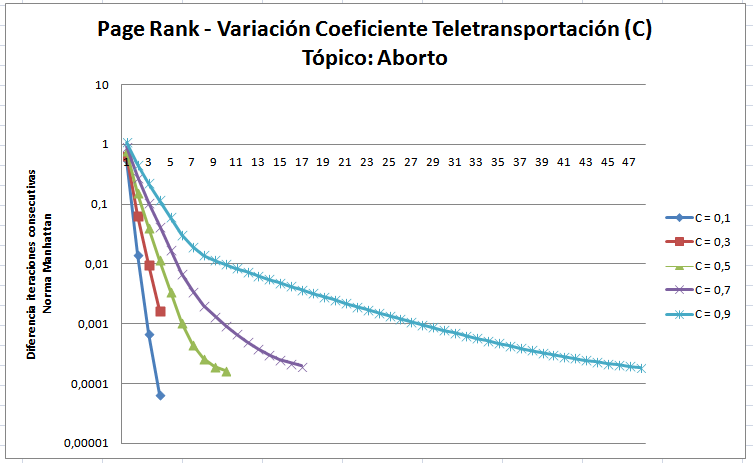
\includegraphics[scale=0.6]{./img/page_rank_variacion_coef_teletransportacion.png}
	\end{center}
	\par 

	Vemos que aumentando el valor de $c$, la cantidad de iteraciones necesarias para obtener un número menor al considerado como $0$ aumenta. Debido a que $c$ impacta tanto en los valores originales de la matriz que eran $0$ como en los que no, podemos pensarlo como la aplicación de un ruido sobre los datos originales. Resulta razonable pensar que a mayor cantidad de ruido, más díficil es al algoritmo encontrar la solución correcta.

	Sin embargo, en la práctica es fáctible y practicable el salto aleatoréo de página en página. Por lo tanto, utilizar un coeficiente muy pequeño, por un lado nos haría tener una solución de manera más rápida; pero por el otro, se generaría un modelo que no se corresponde con nuestro objetivo (cómo generar un \textit{ranking} cualitativo de la red). Los buscadores de internet deben balancear estos dos puntos. Según los artículos leídos, y por lo comentado también en clase, \textit{Google} utiliza un $c = 0.15$, el cuál dado el gráfico supone una buena relación entre \textit{performance} y calidad. 

	Debemos notar que si bien parece que a mayor cantidad de iteraciones mayor error, esto fluctúa con $c = 0.3$. Dado que como recién dijimos el buscador utiliza $0.15$, el cual debería tener una curva similar a la de $0.1$, y que con $0.3$ necesitamos la misma cantidad de iteraciones, pero conseguimos una solución al menos un orden de magnitud menor de calidad; nos preguntamos qué sucede alrededor de esos valores. A continuación, se detallan distintos valores para la teletransportación entre $0.1$ y $0.3$

	\par 
	\begin{center}
		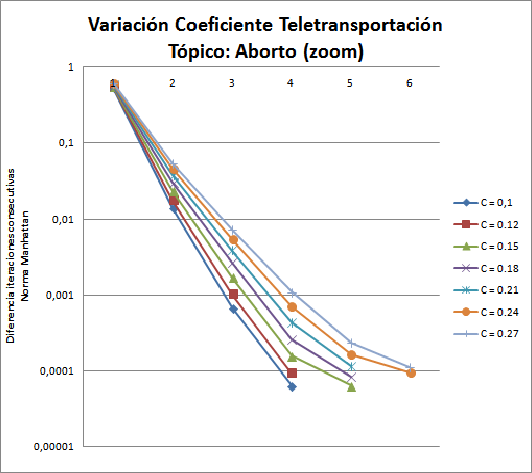
\includegraphics[scale=0.6]{./img/page_rank_variacion_coef_teletransportacion_zoom.png}
	\end{center}
	\par 

	Podemos confirmar que nuesta hipótesis: `` A mayor cantidad de iteraciones, mayor error'', queda refutada. Con 0.15 y 0.1 obtuvimos datos muy similares así como con 0.12 y 0.18. No podemos extraer una función monótona creciente de estos datos. 

	Para nuestro asombro, utilizando el famoso coeficiente 0.15 obtuvimos el mínimo de la muestra tomada. Estrictamente hablando, es un resultado anecdótico, ya que el grafo utilizado no representa la red completa y la semilla para la creación del vector aleatoreo está fija para poder replicar los datos.

	A continuación se incluye el gráfico tomando $c = 1$

	\par 
	\begin{center}
		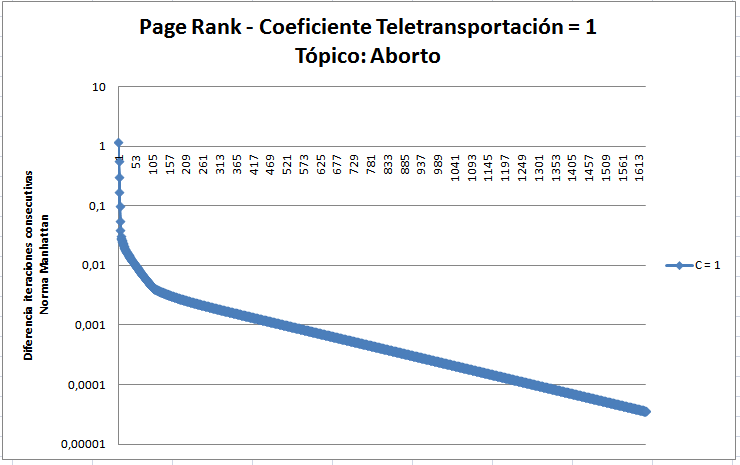
\includegraphics[scale=0.6]{./img/page_rank_variacion_coef_teletransportacion_1.png}
	\end{center}
	\par 

	Por un lado destacamos cómo se elevó la cantidad de iteraciones para coverger. Tomando 0.9 fueron 47, y con 1 más de 1600. Es primordial remarcar que la única información relevante extraíble es que el método de la potencia converge. El vector resultante no tiene por qué estar relacionado con la idea de `` buena solución'', siendo `` buena'' medida cualitativa. Remarcamos esto dado que el grafo de la web no afecta en el cálculo realizado. Si fuera buena solución, sería una mera coincidencia.

	A continuación se realiza la misma prueba que la del primer gráfico, utilizando el set de datos de \textit{genética}. Queremos ver si se observan diferencias en las velocidades de convergencia para refutar nuestras hipótesis anteriores o reforzarlas.

	\par 
	\begin{center}
		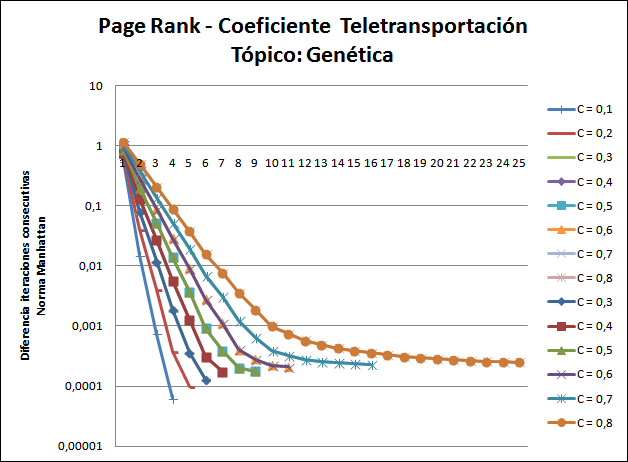
\includegraphics[scale=0.6]{./img/page_rank_variacion_coef_teletransportacion_genetica.png}
	\end{center}
	\par 

	Obtuvimos resultados muy similares, mejor convergencia con $c$ más chico, así como menor cantidad de iteraciones. En este caso no tuvimos el resultado anómalo con $c=0.3$. Atribuímos este resultado a la diferencia en los datos.




\subsubsection{Convergencia de HITS}

El estudio de la convergencia para HITS es muy similar al de \textit{PageRank}, aunque cuenta con una facilidad: no incluye el parámetro $c$. Sin embargo, esta vez necesitamos que el criterio de corte se aplique al mismo tiempo para el vector de pesos de autoridad que para el de pesos de \textit{hub}. Igualmente, esto último no nos supondrá problemas a la hora de analizar la convergencia del algoritmo de búsqueda. Veamos entonces qué sucede para una red mediana-grande al igual que en el estudio de la sección anterior para \textit{PageRank}:
	
	\par 
	\begin{center}
		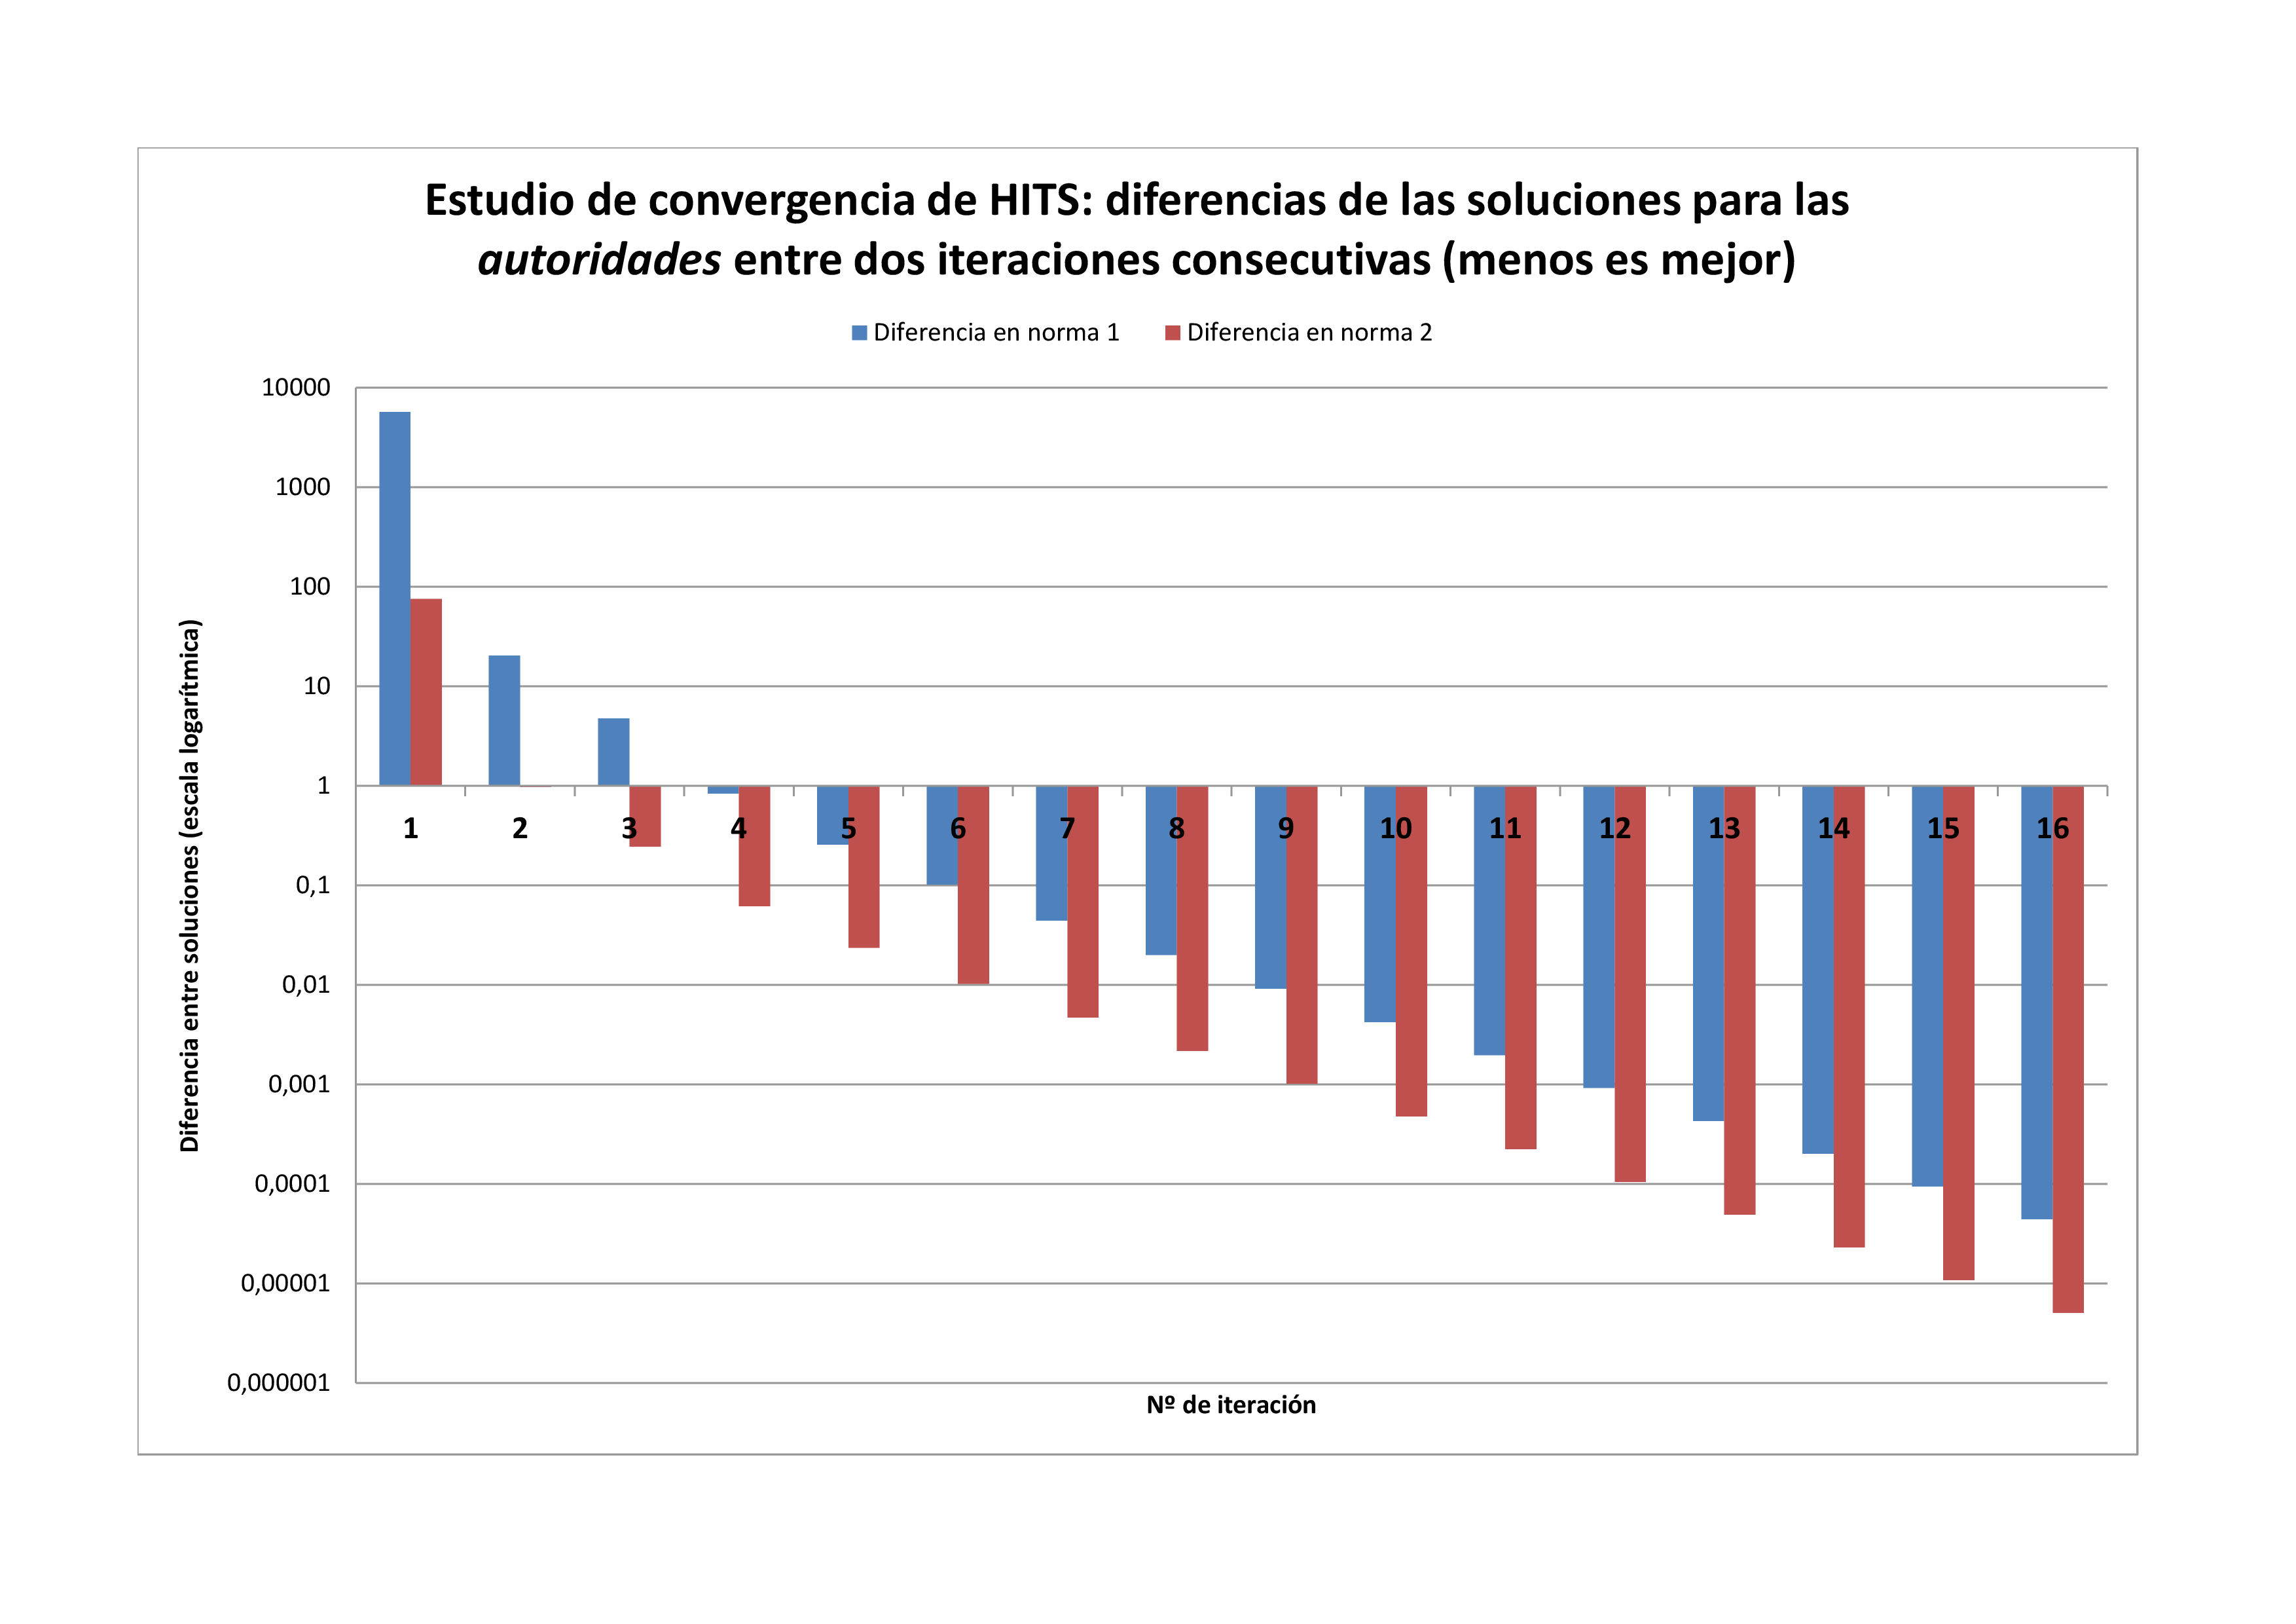
\includegraphics[scale=0.12]{./img/graficoAutoridadesMovies.png}
		\par
		\footnotesize\textit{Estudio de convergencia para HITS para la red de \texttt{movies\_expanded}. Pesos de autoridad.}
	\end{center}
	\par 
	
	Aquí se puede observar el gráfico con las diferencias entre cada solución en cada iteración. Para calcular estas diferencias se utilizó la norma Manhattan (o norma 1, en azul) y la norma 2 (en rojo). La escala en el eje $y$ es logarítmica para una mejor visualización de los resultados. Básicamente, cuanta más diferencia hay en cualquiera de las dos normas, más arriba estarán las barras y viceversa. Por lo tanto, es fácil notar que a medida que se realizan las iteraciones de los productos matriz-vector, menor es la diferencia entre las soluciones de dos iteraciones consecutivas. Esto habla \textit{a priori} de una convergencia a una solución única, justo lo que querríamos encontrar. Veamos qué sucede al mismo tiempo para los pesos de \textit{hub}:
	\par 
	\begin{center}
		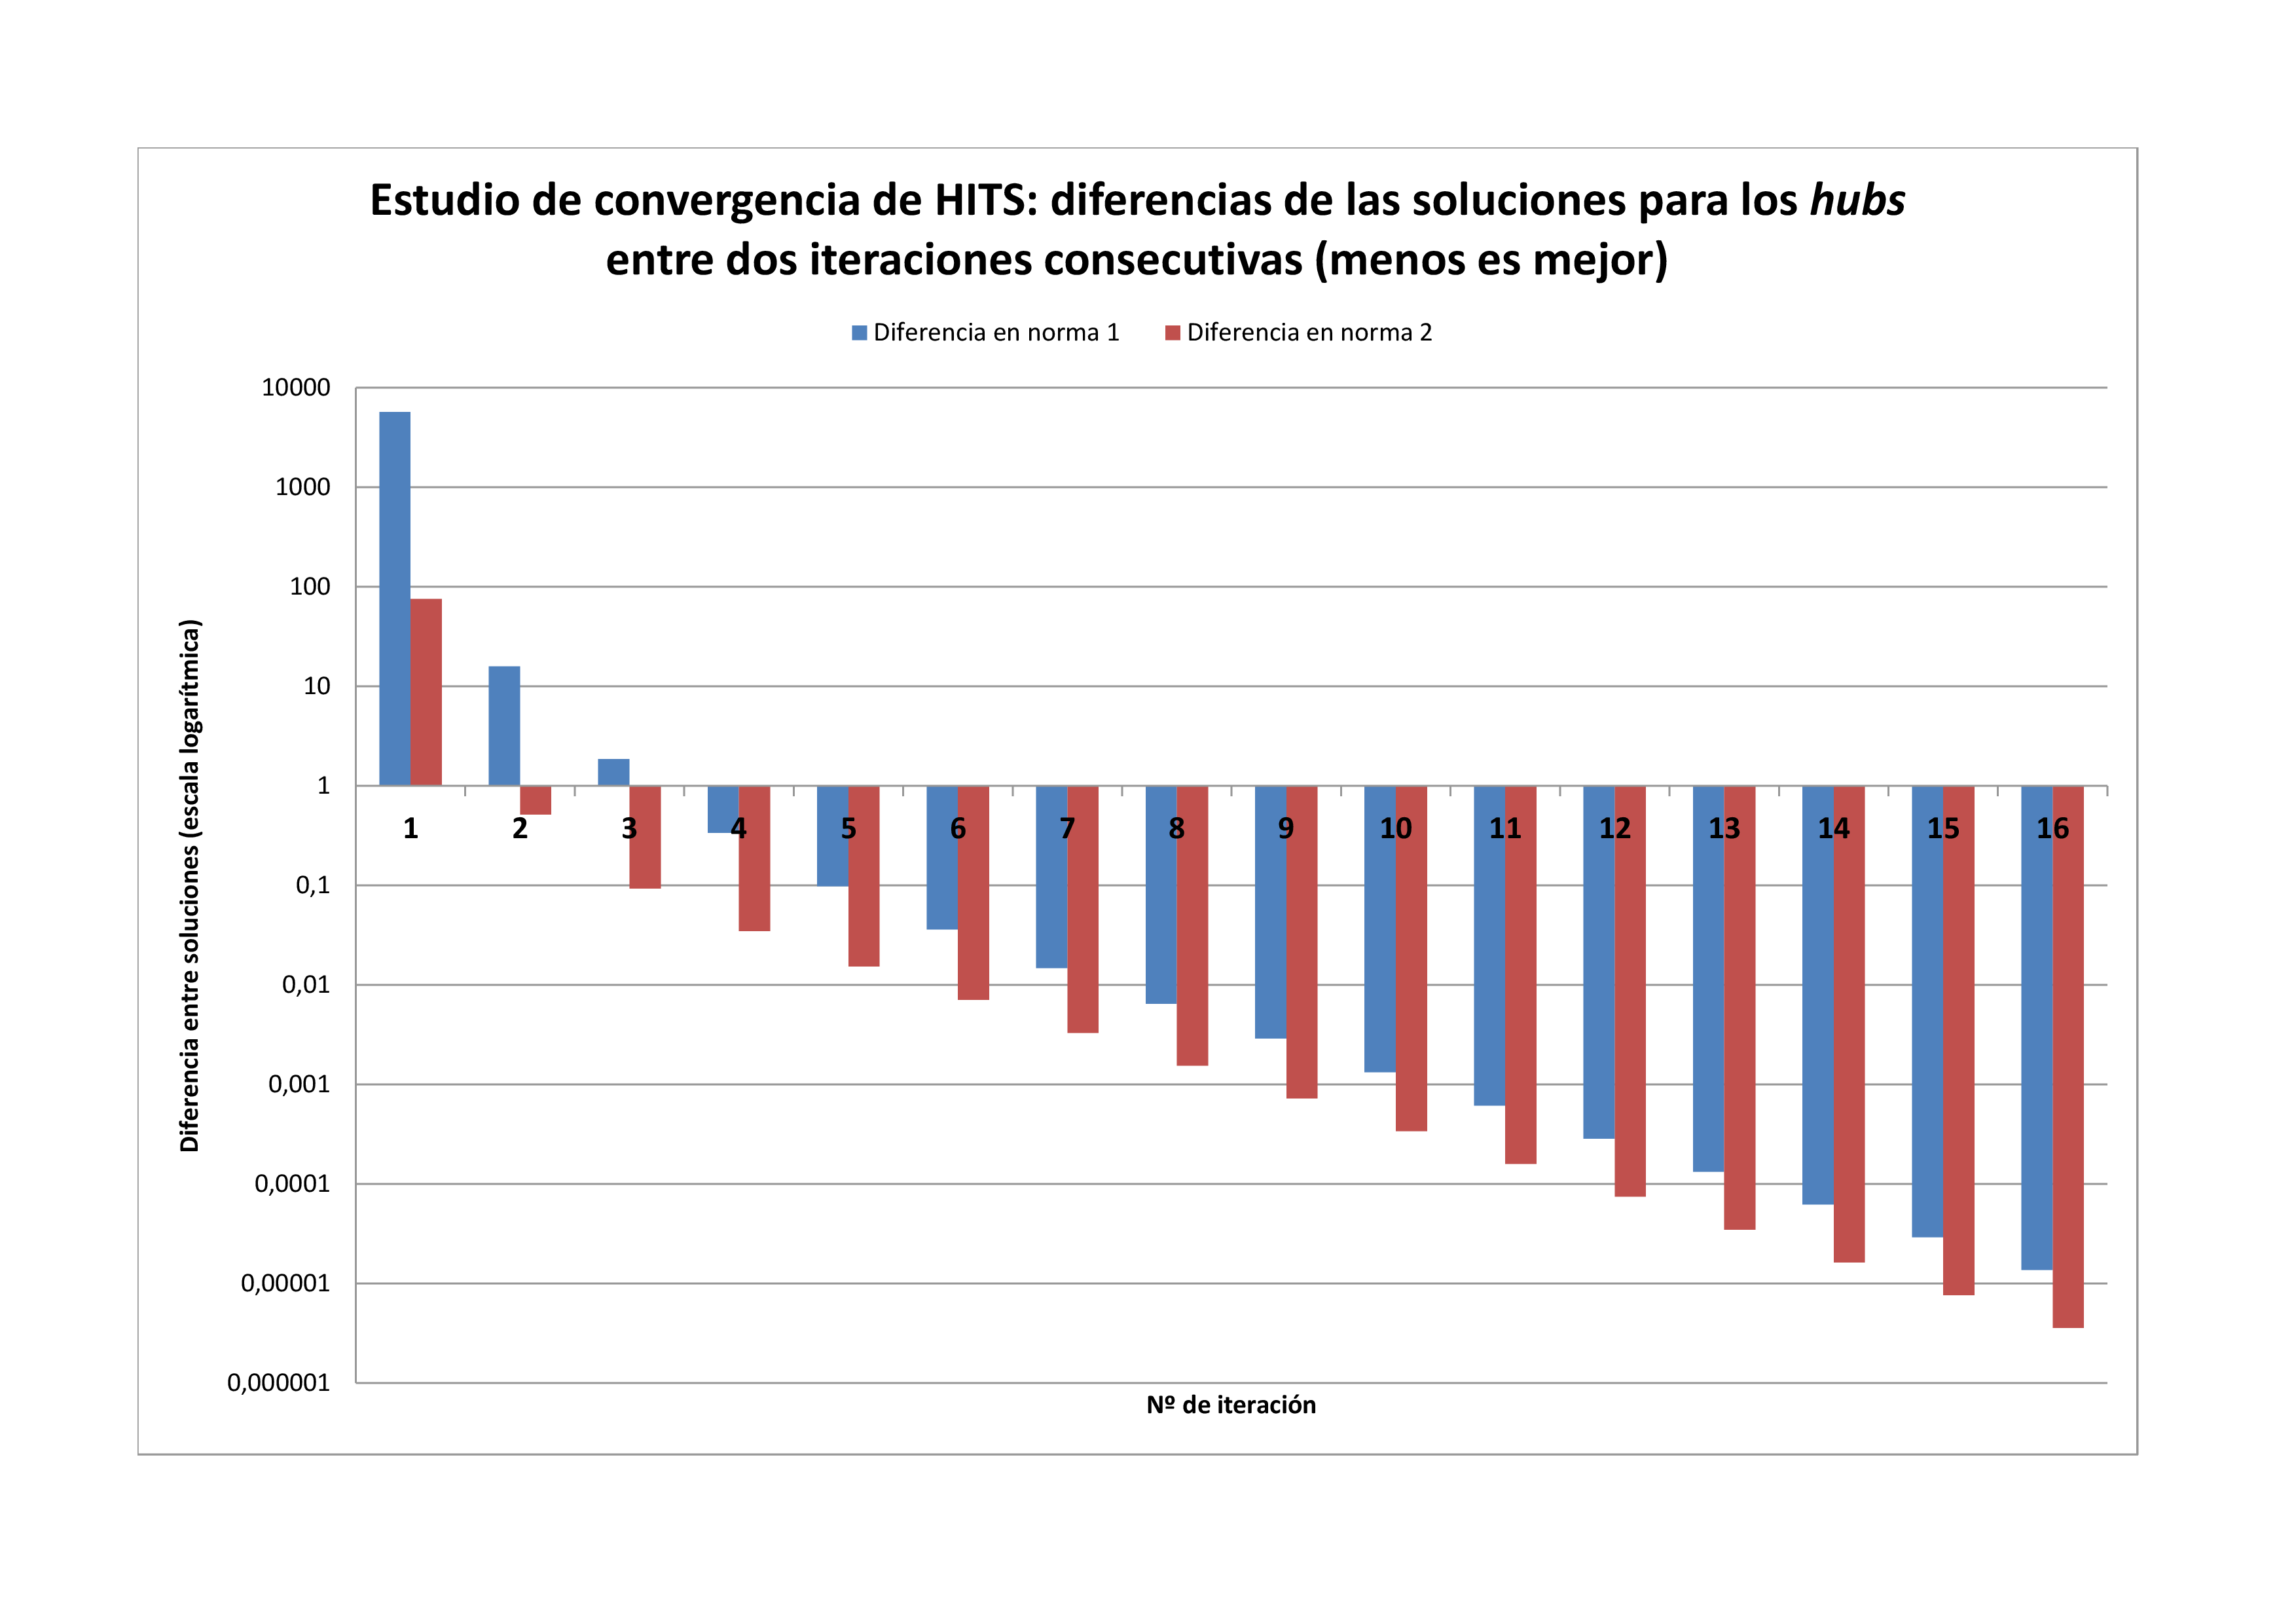
\includegraphics[scale=0.12]{./img/graficoHubsMovies.png}
		\par
		\footnotesize\textit{Estudio de convergencia para HITS para la red de \texttt{movies\_expanded}. Pesos de hub.}
	\end{center}
	\par 
	
	Prácticamente los valores \textit{son los mismos}, no hay cambios notables entre estos pesos y los anteriores: la convergencia para ambos vectores se ve entonces en este caso.
	
	Algunos valores para resaltar en ambos (y en cualquier resultado para una corrida en una red con nuestra implementación de HITS) es por ejemplo aquel de la primera iteración: los vectores iniciales para los pesos son \textit{vectores de unos}\footnote{Siguiendo el paper de Kleinberg, p.9 del PDF función Iterate.}, por lo tanto la diferencia para la primera iteración y el set inicial de vectores es \textit{muy alta} y en particular para la norma Manhattan, \textit{muy parecida a la cantidad de nodos que hay en la red}. En este caso de \textit{movies\_expanded}, había 5757 nodos y la diferencia para la primera iteración está muy cerca de ese número (aprox. 5734 de diferencia para ambos).
	
	\vspace{\baselineskip}
	
	Haciendo más experimentos sobre las bases medianas-grandes que nos ofreció la cátedra nos dimos cuenta de que estos valores \textit{se repetían para todas ellas}. Consideramos adecuado no adjuntar más ejemplos ya que son análogos\footnote{Sin embargo, podrán encontrar en la carpeta de \textit{tests/HITS\_statistics} los demás resultados, con el formato: cantidad de nodos, todos los pesos de autoridad y luego los pesos de hub (en columnas número de iteración, norma 1, norma 2 para ambos).}. Con esto podemos concluír un poco mejor que la convergencia para el algoritmo HITS es un hecho a nivel práctico. Las diferencias están sobre cuán rápido converge (es decir, la cantidad de iteraciones que se realizaron antes de terminar), la cual no supera nunca las 50 iteraciones y suele estar alrededor de 20 iteraciones. Comparando estos valores con los de \textit{PageRank}, podemos intuir desde ya que el tiempo de cómputo será mucho más rápido para HITS porque hace significativamente menos iteraciones. Faltará ver entonces en qué nos beneficia cualitativamente el parámetro $c$ de \textit{PageRank} frente a HITS.
	
	 Algo para destacar de la cantidad de iteraciones es que \textbf{no} depende de la cantidad de nodos de la red. Que el algoritmo HITS utilice más o menos iteraciones dependerá de la tolerancia (fija en $10^{-5}$ para todos los experimentos ya dichos) pero también de cómo se realizan las cuentas y la forma de la matriz de adyacencia y de los vectores iteración por iteración\footnote{Estas formas mencionadas de la matriz de adyacencia y los resultados de cada vector para cada iteración no los pudimos analizar profundamente y por falta de tiempo los dejamos de lado, sintiendo que era una tarea bastante compleja de realizar con las redes propuestas.}. 

\subsubsection{Tiempo de Cómputo}	
Se realizaron mediciones para corroborar la cantidad de ciclos de reloj promedio que ocupa el algoritmo \textit{PageRank} y \textit{HITS}. Estos se realizaron en una ultrabook Exo con procesador Intel Core i7-3517U CPU @ 1.90GHz-2.40GHz, con 8GB de memoria RAM.  
\par 
Con fin de reducir la presencia de outliers y, a su vez, que el costo de cómputo (respecto a tiempo de ejecución) no sea tan amplio, los experimentos se realizaron con 100 iteraciones del algoritmo, obteniendo un promedio de ciclos de reloj por iteración.
\par 
Se tomaron como datos de entrada los archivos brindados por la cátedra en la carpeta \textit{data/query-graphs} y se realizaron las mediciones bajo las condiciones previamente mencionadas.
\par 
A continuación se presenta un primer gráfico. Tener en cuenta que la cantidad de ciclos promedio se presenta en escala logarítmica. 

	\par 
	\begin{center}
		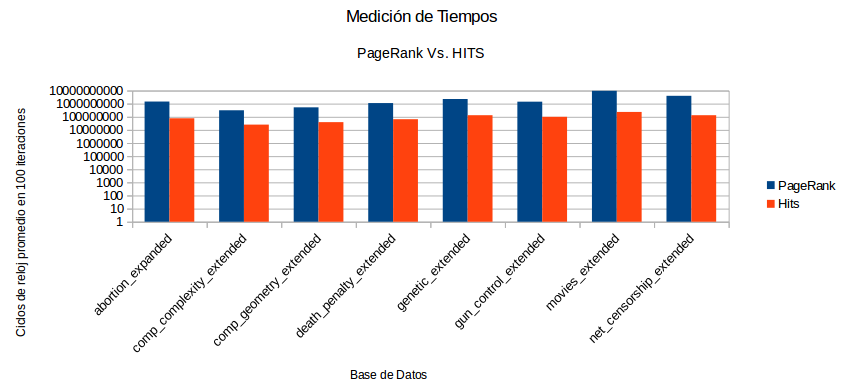
\includegraphics[scale=0.5]{./img/medicionesTiempo1.png}
	\end{center}
	
	\par 

En todos los casos, el promedio de ciclos de reloj es  mayor para el \textit{PageRank}. Se puede notar como, a pesar de que la cantidad de nodos con los que trabajan los algoritmos varía de un conjunto de datos a otro (por lo que el promedio de ciclos de reloj aumenta y disminuye con ella), la relación que hay entre \textit{PageRank} y \textit{HITS} es similar cuantitativamente. Esto quiere decir que, aunque el algoritmo de \textit{PageRank} cueste mayor tiempo en promedio en todos los casos, \textit{HITS} se mantiene siendo aproximadamente $k*10$ veces más rápido siendo $1 \leq k \leq 9$. 
\par 

\begin{center}
    \begin{tabular}{| l | l | l | l |}
    \hline
    Base de Datos & Ciclos PageRank & Ciclos HITS & Cant. Nodos \\ \hline
    $death\_penalty\_extended$ & 1105755584 & 65173039 & 1849 \\ \hline
    $abortion\_expanded$ & 1437873935 & 76885886 & 2292 \\ \hline
	$genetic\_extended$ & 2253042725 & 131592995 & 3467 \\ \hline
	$movies\_extended$ & 9444868351 & 232831140	& 5756 \\ \hline
    \end{tabular}
\end{center}

Como se mencionó previamente, mientras mayor es la cantidad de nodos, mayor es el tiempo de cómputo de ambos algoritmos(se analizará posteriormente). Y a su vez, se puede ver para estos (se aplica para todos), que el valor $k$ propuesto previamente se encuentra entre $1$ y $9$ (es decir, solo hay una diferencia en un factor $10$ y no mayor).
\par 
Por ejemplo, para el caso de la \textit{death\_penalty\_extended}, se puede llegar a que $k \cong 1,6966$. Esto se obtiene haciendo la división entre \textit{cantidad de ciclos de PageRank} y \textit{ciclos de HITS}, para finalmente dividir por $10$. 
\par 
Para el caso de \textit{abortion\_expanded} se obtiene $k \cong 1,8701$, \textit{genetic\_extended} presenta una $ k \cong 1,7121$ y \textit{movies\_extended} un $k \cong 4,0565$, siendo esta la base que mayor $k$ tiene para las queries brindadas por la cátedra. Esto permitiría acotar el $k$ por $5$ para estos caso, pero no es lo que se busca, ya que solo se intenta plantear que el algoritmo de HITS mantiene una relación para cualquiera sea la base con el algoritmo de PageRank respecto al tiempo de cómputo.

Veamos por otro lado un gráfico que permita visualizar si la base afecta en algo al tiempo de ejecución del algoritmo:

	\par 
	\begin{center}
		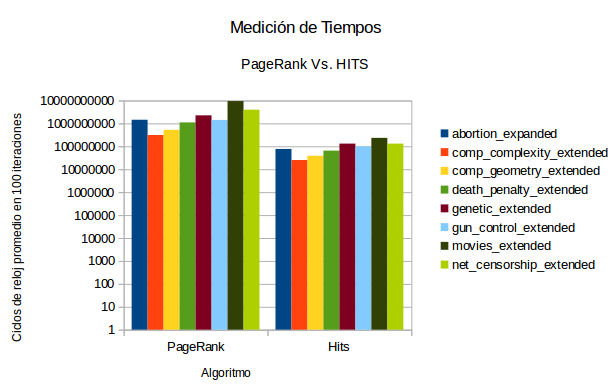
\includegraphics[scale=0.6]{./img/medicionesTiempo2.png}
	\end{center}
	\par 

A pesar de que hay una diferencia considerable entre los tiempos de ejecución para distintos algoritmos, si consideramos la cantidad de ciclos promedio individualmente para \textit{PageRank} y \textit{HITS}, podemos ver que las diferencias entre las distintas bases no es considerable. La misma se produce principalmente por los diferentes tamaños de cada conjunto de datos (como se mencionó previamente). 
A continuación se puede ver la cantidad de nodos en cada base para realizar la comparación. 

\begin{center}
    \begin{tabular}{| l | l | l | l |}
    \hline
    Base de Datos & Ciclos PageRank & Ciclos HITS & Cant. Nodos \\ \hline
    $comp\_complexity\_extended$ & 309975581 & 25232390 & 883 \\ \hline
    $comp\_geometry\_extended$ & 524694925 & 38812606 & 1225 \\ \hline
	$gun\_control\_extended$ & 1413533348 & 99154919 & 2136 \\ \hline
	$genetic\_extended$ & 2253042725 & 131592995 & 3467 \\ \hline
	$movies\_extended$ & 9444868351 & 232831140	& 5756 \\ \hline
    \end{tabular}
\end{center}

En comparación con el gráfico, se puede notar como (con estos casos de ejemplo) el tiempo de cómputo en promedio crece a medida que crece la cantidad de nodos. Esto tiene sentido ya que, al ser mayor la cantidad de nodos, las matrices de adyacencias utilizadas son más grandes, lo que inevitablemente conlleva a un mayor tiempo de ejecución.

\par 

En conclusión, el algoritmo de \textit{PageRank} tiene mayor tiempo de cómputo. En este sentido, para casos de tamaño mediano a grande, sin realizar un análisis de calidad de la solución (el cual se hará posteriormente en este trabajo práctico), \textit{HITS} parece comportarse mejor. Sin embargo, hay que tener en cuenta que parte del proceso de este algoritmo (como es la realización del subgrafo de la red) no es realizado por nuestra implementación por lo que se reduce el tiempo de cómputo. 
\par A pesar de esto, la amplia diferencia en cantidad de ciclos de ambos algoritmos reflejan los usos que poseen ambos. Por un lado, \textit{PageRank} puede ser mejor utilizado como un proceso batch que se ejecuta cada cierto período de tiempo y no en el momento, mientras que \textit{HITS} es un algoritmo pensado para realizar el rankeo en el momento sobre un subgrafo de la red. De esta manera, tiene sentido que el algoritmo \textit{HITS} sea más veloz que el algoritmo de \textit{PageRank}, nuevamente, sin tener en cuenta en ningún momento la calidad del resultado.



\subsubsection{Análisis Cualitativo}
Luego de realizar un análisis cuantitativo en la sección previa, es necesario preguntarnos si el resultado obtenido por estos algoritmos es considerado correcto. 
Para esto, hay que preguntarnos ¿Qué es la calidad en una búsqueda? 
\par 
Para realizar un análisis cualitativo decidimos tomar algunos reconocidos motores de búsqueda como son \textit{google}, \textit{yahoo} y \textit{bing}, y tratamos de recrear una búsqueda que otorgue como resultado varias de las páginas que se encuentran en el archivo \textit{weblist.in}. Es por esto que se eligió realizar la búsqueda ``diarios argentinos'' ya que en el mencionado archivo se podrían encontrar varios de estos links bajo esa búsqueda.
\par 
Para esto, primero veamos cuales fueron los resultados obtenidos por nuestros algoritmos. Empecemos con \textit{pageRank}. A continuación presentamos los datos obtenidos luego de ejecutar el algoritmo con una probabilidad de transportación de $0,10$ y una tolerancia de corte de $0.00001$. Se presenta la información ordenada decrecientemente por ranking:

\begin{center}
    \begin{tabular}{| l | l | l |}
    \hline
    Posición & Página & Rank  \\ \hline
    
	1 & www.clarin.com & 0.0788695 \\ \hline
	2 & www.ole.com.ar & 0.0782334 \\ \hline
	3 & www.lanacion.com.ar & 0.0779999 \\ \hline
	4 & www.clasificados.clarin.com & 0.073492 \\ \hline
	5 & www.ciudad.com.ar & 0.073492 \\ \hline
	6 & canchallena.lanacion.com.ar & 0.0732727 \\ \hline
	7 & www.rollingstone.com.ar & 0.0697836 \\ \hline
	8 & www.zonaprop.com.ar & 0.0697836 \\ \hline
	9 & www.clarin.com/deportes & 0.0691553 \\ \hline
	10 & www.google.com & 0.0671836  \\ \hline
	11 & www.pagina12.com.ar & 0.0671836	\\ \hline		
	12 & www.yahoo.com & 0.0671836 \\ \hline
	13 & www.infobae.com & 0.0671836 \\ \hline
	14 & www.mamapuntocero.com.ar & 0.0671836 \\ \hline   
    \end{tabular}
\end{center}

Dado que la búsqueda se realizó sobre ``diarios argentinos'', sería esperable que se obtengan páginas como \textit{www.clarin.com}, \textit{www.ole.com.ar}, \textit{canchallena.lanacion.com.ar} o \textit{www.pagina12.com.ar} mientras que otras como pueden ser \textit{www.yahoo.com} o \textit{www.google.com}. 
\par 
De esta manera, luego se comenzó realizando la búsqueda en el motor de búsqueda por excelencia y contra el cual todos deberían compararse: Google.
El mismo arrojo los siguientes resultados:

	\par 
	\begin{center}
		
\includegraphics[scale=0.5]{./img/primerapaginagoogle.png}
	\end{center}
	\par 


\subsubsection{Casos de Ejemplo}
	
	
\section{Conclusión}


\section{Bibliografía y referencias} %arreglar cuando se termine 

\begin{itemize}
	\item \textbf{STL de C++}: \url{http://en.cppreference.com}.
%	\par Para la función \texttt{rand()}, \url{http://en.cppreference.com/w/cpp/numeric/random/rand}.
%	\par Para la función \texttt{sort()}, \url{http://en.cppreference.com/w/cpp/algorithm/sort}.
%	\item Distribución de \texttt{rand()}?, \url{http://eternallyconfuzzled.com/arts/jsw\_art\_r and.aspx}
	\item \textbf{Métodos Numéricos:}
		\par Método de la potencia: Richard BURDEN, Numerical Analysis 9th Ed. Chapter 9 Section 3, p. 576
		\par Papers del TP.
	\item \textbf{Contador de clocks}: \url{http://www.mcs.anl.gov/\~kazutomo/rdtsc.html}
\end{itemize}


\end{document}
